%%%%%%%%%%%%%%%%%%%%%%%%%%% asme2e.tex %%%%%%%%%%%%%%%%%%%%%%%%%%%%%%%
% Template for producing ASME-format articles using LaTeX            %
% Written by   Harry H. Cheng                                        %
%              Integration Engineering Laboratory                    %
%              Department of Mechanical and Aeronautical Engineering %
%              University of California                              %
%              Davis, CA 95616                                       %
%              Tel: (530) 752-5020 (office)                          %
%                   (530) 752-1028 (lab)                             %
%              Fax: (530) 752-4158                                   %
%              Email: hhcheng@ucdavis.edu                            %
%              WWW:   http://iel.ucdavis.edu/people/cheng.html       %
%              May 7, 1994                                           %
% Modified: February 16, 2001 by Harry H. Cheng                      %
% Modified: January  01, 2003 by Geoffrey R. Shiflett                %
% Use at your own risk, send complaints to /dev/null                 %
%%%%%%%%%%%%%%%%%%%%%%%%%%%%%%%%%%%%%%%%%%%%%%%%%%%%%%%%%%%%%%%%%%%%%%

%%% use twocolumn and 10pt options with the asme2e format
\documentclass[twocolumn,10pt]{asme2e}
\usepackage[utf8]{inputenc}
\usepackage{epsfig}
\usepackage{subfigure}
%% The class has several options
%  onecolumn/twocolumn - format for one or two columns per page
%  10pt/11pt/12pt - use 10, 11, or 12 point font
%  oneside/twoside - format for oneside/twosided printing
%  final/draft - format for final/draft copy
%  cleanfoot - take out copyright info in footer leave page number
%  cleanhead - take out the conference banner on the title page
%  titlepage/notitlepage - put in titlepage or leave out titlepage
%  
%% The default is oneside, onecolumn, 10pt, final

%%% Replace here with information related to your conference
\confshortname{ESDA 2012}
\conffullname{the ASME 2012 11th Biennial Conference On Engineering Systems Design \\ And Analysis}

%%%%% for date in a single month, use
\confdate{2-4}
\confmonth{July}
%%%%% for date across two months, use
%\confdate{August 30-September 2}
\confyear{2012}
\confcity{Nantes}
\confcountry{France}

%%% GM: overcome bullet list issues (see FAQ)
\newcommand\labelitemi{\textbullet}

%%% Replace DETC2010/MECH-12345 with the number supplied to you 
%%% by ASME for your paper.
\papernum{ESDA2012-82141}

%%% You need to remove 'DRAFT: ' in the title for the final submitted version.
\title{MARKUS, AN OPEN-SOURCE WEB APPLICATION TO ANNOTATE STUDENT PAPERS ON-LINE}

%%% first author
\author{Karen Reid
    \affiliation{
	University of Toronto\\
	40 St. George St.\\
	Toronto, Ontario M5S 2E4\\ 
	Canada\\
    Email: reid@cs.toronto.edu
    }	
}

\author{Mike Conley
    \affiliation{
	Mozilla Corp.\\
	Canada\\
    Email: mike.d.conley@gmail.com
    }	
}

\author{Severin Gehwolf
    \affiliation{
	University of Toronto\\
	40 St. George St.\\
	Toronto, Ontario M5S 2E4\\ 
	Canada\\
    Email: severin.gehwolf@utoronto.ca
    }	
}

\author{Morgan Magnin \\
       {\tensfb Guillaume Moreau}   
    \affiliation{
	LUNAM Universit\'{e} \\
	Ecole Centrale de Nantes\\
	1 rue de la No\"{e}, BP 92101\\
	44321 Nantes Cedex 3\\
	France\\
    Email: morgan.magnin@ec-nantes.fr \\
    guillaume.moreau@ec-nantes.fr
    }	
}


\author{Nelle Varoquaux
    \affiliation{
	Affiliation ?\\
    Email: nelle.varoquaux@gmail.com
    }	
}

\author{Benjamin Vialle
    \affiliation{
	Mobile Devices Ingenierie\\
	100, avenue de Stalingrad\\
	94800 Villejuif\\
		France\\
    Email: benjaminvialle@gmail.com
    }	
}

\begin{document}

\maketitle    

%%%%%%%%%%%%%%%%%%%%%%%%%%%%%%%%%%%%%%%%%%%%%%%%%%%%%%%%%%%%%%%%%%%%%%
\begin{abstract}
{\it A critical component of the learning process lies in the feedback that students receive on their work that validates their progress, identifies flaws in their thinking, and identifies skills that still need to be learned. Many higher-education institutions have developed an active pedagogy that gives students opportunities for different forms of assessment and feedback. This means that students have numerous lab exercises, assignments, and projects. Both instructors and students thus require effective tools to efficiently manage the submission, assessment, and individualized feedback of students' work. The open-source web application MarkUs aims at meeting these needs: it facilitates the submission and assessment of students' work. Students directly submit their work using MarkUs, rather than printing it, or sending it by email. The instructors or teaching assistants use MarkUs's interface to view the students' work, annotate it, and fill in a marking rubric. Students use the same interface to read the annotations and learn from the assessment. Managing the students' submissions and the instructors assessments within a single online system, has led to several positive pedagogical outcomes: the number of late submissions has decreased, the assessment time has been drastically reduced, students can access their results and read the instructor's feedback immediately after the grading process is completed. Using MarkUs has also significantly reduced the time that instructors spend collecting assignments, creating the marking schemes, passing them on to graders, handling special cases, and returning work to the students.

%GM: I suggest to remove this paragraph of the abstract in full paper
MarkUs was created and developed at University of Toronto (UofT), Canada. Since summer 2009, students at École Centrale de Nantes (ECN) have joined the MarkUs development team. In use at UofT, University of Waterloo (Canada) and ECN, MarkUs supports the assessment of several thousand students.

In this paper, we introduce MarkUs' features, and illustrate their benefits for higher education through our own teaching experiences and that of our colleagues. We also describe an important benefit of the fact that the tool itself is open-source. MarkUs has been developed entirely by students giving them a valuable learning opportunity as they work on a large software system that real users depend on. Virtuous circles indeed arise, with former users of MarkUs becoming developers and then supervisors of further development.

We will conclude by drawing perspectives about forthcoming features and use, both technically and pedagogically.}
\end{abstract}

%%%%%%%%%%%%%%%%%%%%%%%%%%%%%%%%%%%%%%%%%%%%%%%%%%%%%%%%%%%%%%%%%%%%%%
%\begin{nomenclature}
%\entry{A}{You may include nomenclature here.}
%\entry{$\alpha$}{There are two arguments for each entry of the nomemclature environment, the symbol and the definition.}
%\end{nomenclature}

%The spacing between abstract and the text heading is two line spaces.  The primary text heading is  boldface in all capitals, flushed left with the left margin.  The spacing between the  text and the heading is also two line spaces.

%%%%%%%%%%%%%%%%%%%%%%%%%%%%%%%%%%%%%%%%%%%%%%%%%%%%%%%%%%%%%%%%%%%%%%
\section*{INTRODUCTION}

% The main idea : Why is assessing student papers so important, why there are so many difficulties when many students and teachers are involved, how every one of us previously tried to manage with these difficulties, why a tool like MarkUs was needed

Assessing and providing feedback on student work is a critical and time consuming component of any course. It is especially true in computer science training. Receiving timely, high quality feedback is a important pedagogic goal of any course. MarkUs is designed to simplify the process of submitting work, provide an intuitive interface to annotate students work and record grades, and reduce the administrative task of the instructors. 

With all types of work submitted by students there are a number of steps involved.

\begin{itemize}
        \item Submissions. Students use some mechanism to submit their work either on paper or electronically.
        \item Assessment.  Some form of grading scheme is used to evaluate the students' work.
        \item Feedback. The graders provide feedback in the form of general comments or annotations on the students' work.
        \item Distribution. The work is returned to the student with the grade and the feedback.
        \item Record keeping. The instructor collects the grades to determine a final evaluation.
\end{itemize}

Of these steps the most challenging is to provide high quality feedback efficiently. While there are many advantages to submitting work electronically, it is challenging to provide the kind of simple efficient feedback achieved by circling incorrect work or drawing a few arrows directly on a paper submission. One of our previous attempts simplified the management and evaluation of work submitted electronically by students through the use of Tablet PCs \cite{magnin-tice-2010}. Although this approach facilitated annotating their work, the management of students' submission still remained a hot topic: in the past, we received files by e-mail, temporarily stored on the instructor's computer then returned them corrected to the sender(s). This method is error prone, time consuming and only works for small to medium class sizes. Another solution to collect students' work was the use of the submission tools provided by the submission tools of elearning platforms such as Claroline~\cite{claroline} or Moodle~\cite{moodle}. Yet practical to handle numerous submissions and marking, there tools could not be used to handle  annotation of the students' work thus motivating us to turn to a new relevant and effective tool for the assessment of students' work: MarkUs \cite{markus}.

MarkUs was created at University of Toronto (UofT), Canada. Since summer 2009, students at Ecole Centrale de Nantes (ECN) have joined the MarkUs development team. First used at UofT in September 2009, and at the University of Waterloo (Canada) in January 2010, MarkUs was deployed at ECN in September 2010. In this paper, we present MarkUs' features, and illustrate their potential assets for higher education through our own feedback. We will not only provide an overview of current uses and future but also put the emphasis on the benefit taken from the fact that such a tool is open-source. 

MarkUs takes into account the needs expressed by teachers and students. Encompassed in a single web-application, the primary features of MarkUs follow:
\begin{itemize}
\item Students submit documents using MarkUs. This has the advantage that graders and instructors do not need to manage submissions via email, or copy submissions around. Documents are versioned (i.e., successive versions of each file are stored), so that teachers can track the progress of students over time \cite{Reid05learningby}. Students can easily see exactly what they submitted, allowing them to check their work.
\item Graders view student documents and add annotations within MarkUs. They also fill in a grading scheme created by the instructor. 
\item A standard set of reusable annotations may be created ahead of time, and graders may save annotations for later reuse.
\item The software manages the deadlines that students must respect to submit their work. It is possible to specify additional features, like ``grace period credits" or ``penalty formulas";
\item When the grading of an assignment or piece of work has been completed, the instructor can ``release'' the grades to the students.
\item Students view their grades and feedback through a read-only view of the same interface graders used to generate the feedback.
\item Instructors may download grades for further processing.
\end{itemize}

Additional features are described in the next section.

%Students no longer need to print their code, or send it by email to their teachers: all these steps are managed via MarkUs, which recreates the ease and flexibility of grading assignments with pen on paper. 

In this paper, we will first describe the core MarkUs features as well as more recent enhancements. Then we will detail how MarkUs has been deployed in various Canadian and French institutions, allowing us to analyze the impact of this new software in the whole pedagogical process. Finally, we will preview the forthcoming features we plan to integrate in the tool, allowing us to overcome current limitations of the software. 



%%%%%%%%%%%%%%%%%%%%%%%%%%%%%%%%%%%%%%%%%%%%%%%%%%%%%%%%%%%%%%%%%%%%%%
\section*{THE MARKUS TOOL}

% Presentation of the history, then features, of MarkUs

% If the heading should run into more than one line, the run-over is flush left.

%%%%%%%%%%%%%%%%%%%%%%%%%%%%%%%%%%%%%%%%%%%%%%%%%%%%%%%%%%%%%%%%%%%%%%
\subsection*{History}

Initiated during the summer 2005 as Online Marking Tool (OLM), the project aimed
at improving the effectiveness and efficiency of marking lower year Computer
Science assignments. Built using the Python web framework Turbogears, OLM
provided an environment to facilitate grading programming assignments online including the ability to annotate student work, and fill in a marking rubric. During its three-year deployment at the UofT, we learned the strengths and weaknesses of OLM. The ``grader view'', which allowed TAs to annotate and asses the student submissions was very successful, but the administrative overhead was high and we could see many opportunities to improve the user interface for graders. Our plans to extend and enhance OLM were hampered by a decaying code base, lack of adequate tests, and a sense that modern web programming frameworks would be more advantageous to the project.

In the summer of 2008, it was decided to rewrite the whole application in Ruby on Rails. We kept the best features of OLM as MarkUs took shape, but MarkUs included many new features. One year later, MarkUs was deployed for the first time as a replacement to OLM. Thanks to more careful software development practices, including extensive testing and code reviews, the first deployment of MarkUs went very smoothly.

\subsection*{Free software philosophy}
MarkUs is free software, i.e. a software whose use, study, editing and duplication for distribution are permitted, technically and legally, to guarantee a wide range of freedoms to the end-user. Licensed under the MIT Open Source License, it is developed mainly by Canadian and French students.

Presented at several conferences, MarkUs receives various outside contributions. Students and teachers from other universities send patches that are integrated with the main branch of development. The presentations in conference can also expand the range of returns on software, and identify additional needs.

MarkUs benefits from the integration of many components that are widely used in the free software community: a version control module to collect the student code, the use of a well-known javascript library to annotate images and PDF documents, the integration of annotations in LaTeX and MathML to adapt the tool to the research environment. 

\subsection*{Community}
MarkUs is the subject of ongoing developments. Each semester, a dozen  new students participate in the implementation of its features. They are co-supervised by teachers and technical mentors (that often are former students who continue to participate in the evolution of the software).

Since 2008, more than 45 undergraduate students have participated in the development of MarkUs; some as full-time summer interns, but most working part time on MarkUs as a project course. The fact that we have have uncovered so few major bugs, and that MarkUs has been so well-received by instructors is a testament to the high quality work of these students.

FIXME: Should we add something about ReviewBoard here?

In September 2010, MarkUs's code moved to the public hosting web-service,
GitHub. Allowing any contributor to patch and improve the project's code base has opened MarkUs is to a wider community.

As the development of MarkUs takes profit from the dynamics of project-based learning, we have been able to establish virtuous circles: students, who were former MarkUs users, are invited to become contributors, and then act as technical mentors for new projects once they have been graduated. This positive cycle has been extensively described in \cite{magnin-qpes-2011}.

\subsection*{Features}
\label{features}
%Global presentation of the main MarkUs features

As a web-application, MarkUs is cross-platform (Windows, Mac OS X, Linux,
etc.). As MarkUs can be used through any web browser, it is therefore
well-suited to nomadism situations that students and faculty members may
encounter in their daily life. MarkUs features are summarized in Figure~\ref{fig:features}.

Instructors can enforce submission deadlines, marking schemes, automatic
penalties, and group and grader management (max and min number of students per
groups, who grades which student group or what part of the assignment).

Once the assignment is properly set up, students can start forming groups by
inviting other students, accepting or rejecting invitations. When group
requirements are met, they can start submitting their source code, diagrams,
pictures and schemas on MarkUs. In order to handle automatic version control,
a subversion repository is plugged in the backend of the webfile upload. For
more advanced courses, direct command line access to the repository is
possible.

After the due date is passed, graders can easily annotate students' code,
diagrams and pictures. MarkUs allows instructors to create annotation
categories, load default annotations and graders to save some. Hence, graders
do not need to retype commonly used comments. In order to facilitate
consistent grading, two marking schemes are available: a criteria based one,
or a flexible grading system.

On the fly feedback on grades is given to instructors, allowing marking
schemes readjustments. When grades are released, students can view feedbacks
and marks of assignments online, or download a PDF version.

\begin{figure*}[htbp]
	\centering
		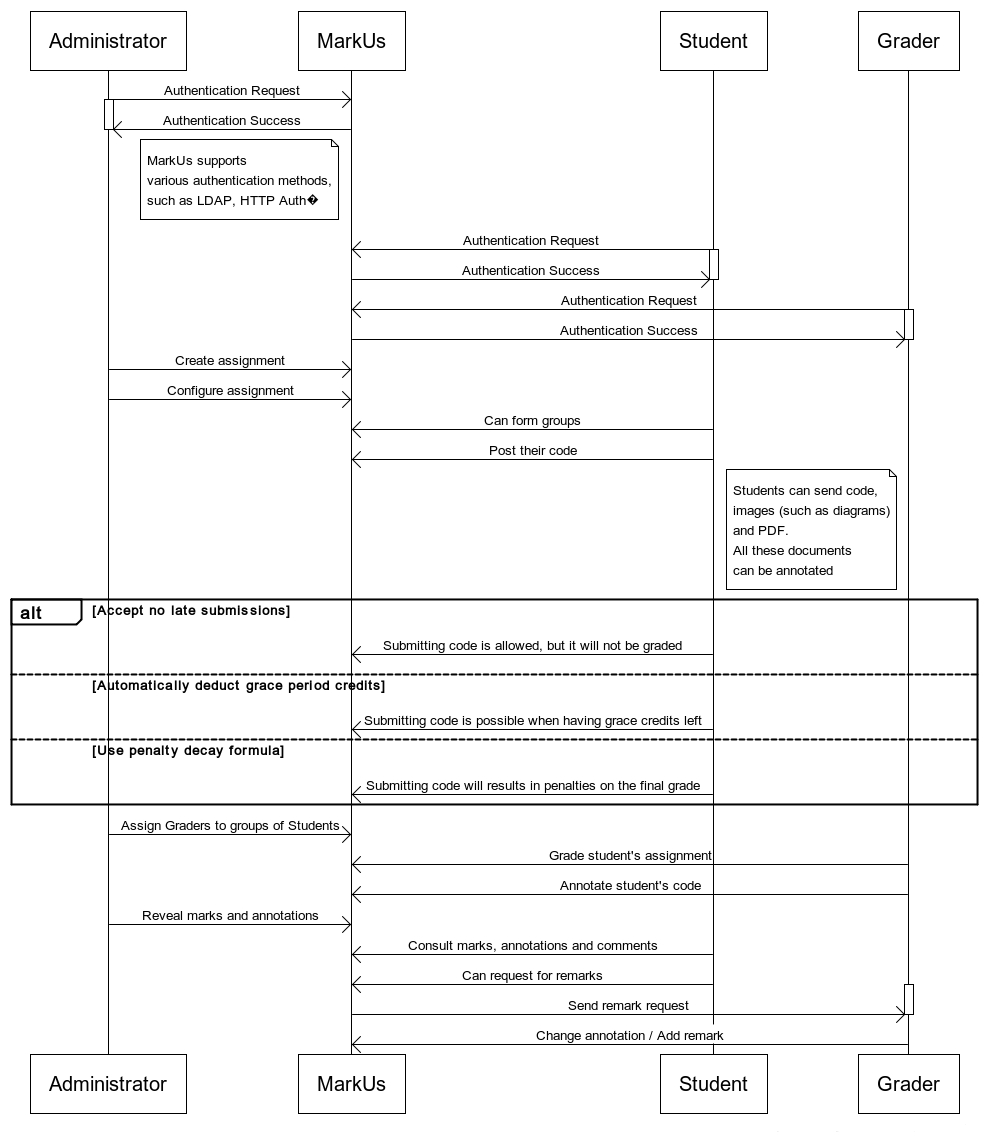
\includegraphics[width=0.95\textwidth]{Diagrams/diagram.png}
	\caption{MarkUs features.}
	\label{fig:features}
\end{figure*}

%%% Add one screenshot of MarkUs, maybe about annotation of code

%%%%%%%%%%%%%%%%%%%%%%%%%%%%%%%%%%%%%%%%%%%%%%%%%%%%%%%%%%%%%%%%%%%%%%
\section*{THE DEPLOYMENT OF MARKUS}

MarkUs has been used in Computer Science related courses since 2007 in Canada and since 2010 in France. In this section, we will detail how students and teachers get used to the tool.

\subsection*{An overview of the use of MarkUs in Higher Education}

MarkUs is currently used at the University of Toronto, University of Waterloo and Ecole Centrale de Nantes: 
%\begin{itemize}
%\item In University of Toronto, ... %to be filled with info about the number of students and courses impacted
%\item In University of Waterloo, ... %to be filled with info about the number of students and courses impacted
%\item In Ecole Centrale de Nantes, MarkUs has been used since 2010. 
MarkUs impacts both undergraduate and master students, in Computer Science related courses like: algorithmics, C and Java programming, databases, modeling languages (UML). Every year, that is an average of 800 students and 20 teachers that use MarkUs in each of the aforementioned institutions. %to be completed
%\end{itemize}

%GM: I suggest to remove the following paragraph
During the last semester, we have been contacted by teachers from various Universities and engineering schools. These teachers would like to give a try to MarkUs in order to overcome the limits of their existing grading process. We are currently helping them in order to make their use be as successful as ours. 

\subsection*{How teachers are accompanied to use the tool? How they use it?}

MarkUs is easy to handle, thus its use does not require a long formation. It
is provided with an extensive documentation, available in both English and
French. This documentation has been structured so that the head-teacher,
teachers and students can find the information they are looking for. There are
as many documentation cases as these three situations, meaning we have a
manual for administrators (which should be the head of a course), graders
(i.e. teachers) and students. 

In our institutions, there are one or two teachers that play the role of "referees" for the software, meaning that every encountered issue can be forwarded to them. Thanks to their knowledge about MarkUs, they can help their fellow teachers with problems that can be overcome. When the issue is an unknown one, they can contact the development team, that may open a ticket. It is fundamental to have these people as interfaces with the development team, allowing to synthesize feedback and give hints about awaited features. 

%%%%%%%%%%%%%%%%%%%%%%%%%%%%%%%%%%%%%%%%%%%%%%%%%%%%%%%%%%%%%%%%%%%%%%
\section*{THE IMPACT OF MARKUS}

The introduction of a new tool in a pedagogical process needs to be monitored in order to get a relevant overview of its advantages and drawbacks. In this section, we will describe the key factors we have identified and how they have been impacted by MarkUs. 

%How the learning process gets improved? How can it be measured? (facts, like: number of students submitting after the deadline; comparisons between the time taken by teachers to comment students works - we have this kind of info from the use if MarkUs by our teachers here at Centrale Nantes, ?)

\subsection*{Analysis criteria}

We evaluate the benefit of MarkUs according to several criteria, that are following: 
\begin{itemize}
\item Quantitatively: how much does MarkUs increases the speed of the assessment process, how it enhances the number of individual comments left on each students' paper, how students' final evaluation improves thanks to the use of MarkUs during courses;
\item Qualitatively: through annual surveys of teachers and students to validate the adequacy of the tool to teachers' needs, the improvement of teaching and the efficiency in the assessment process.
\end{itemize}

Thanks to these analysis processes, we have collected the following key figures: 
\begin{itemize}
\item Thanks to MarkUs, all teachers spend less time to assess the same quantity of students' papers. This time has decreased from a percentage between 14\% and 50\%, depending on the teacher. 
\item The number of students submitting their work after the deadline has drastically decreased: before MarkUs has been adopted, this number was between 15\% and 20\% (students argued there was a misunderstanding about the final deadline, or that they have problems with their emails, \dots).  Now, this number is between 5\% and 10\%. As students know the submission deadline is now an automatic process, they do not try anymore to cheat with this constraint. 
\item There has been a reduction over the number of students' practical work reports that are sent back after the final exam (this number has been divided by 2). As the whole grading process has been made easier and faster, teachers are more willing to do this assessment than before. 
\end{itemize}

These factors have reinforced the idea that MarkUs was responding to needs that have been expressed for many years. It naturally fits into the learning context, it is easy to handle and, finally, it improves the understanding of students w.r.t. the reports and works they have to prepare (ability to get a personal comment on the submitted work, respect of deadlines, etc.).

\subsection*{Results}

MarkUs is a tool that makes life easier for students and graders thanks to a wide range of useful features, such as: the centralized and versioned submission of the papers, its assessment, the annotation of the code and images/PDF documents directly from the web interface, the possibility to download the documents on his own computer to test the code of the students, etc.. As all these  features have been developed specifically for the educational context, MarkUs improves the global pedagogical quality: it offers the possibility to share annotations among multiple teachers and incorporates a correction (and notation) grid defined by the head-supervisor. It also provides an additional organizational element: it is easy and quick to make corrections on large cohorts (e.g. by using "reference annotations" that just copy / paste the most recurrent mistakes) and it is therefore more motivating for teachers. As a noticeable side effect compared with traditional organization of practical sessions in computer science course, there has been a drastic decrease in the amount of paper that is used. 

\subsection*{Analysis of the impact}

Students have become much more respectful of deadlines than they were before, thanks to the fact of not being able to submit the papers once the due date is past. MarkUs has raised more interest to the annotations left on the platform. In addition, students have appreciated the increased speed correction from their teachers. 

As far as the educational team is concerned, MarkUs has helped to unify the criteria for marking groups: even if a large number of students do not have the same teachers, their work is assessed according to the same criteria grid. 

\subsection*{Dissemination}

MarkUs is developed through a strong international collaboration between three institutions of higher education. These institutions include research laboratories. The philosophy of the research is rooted in the DNA of the software. MarkUs follows a development process perfectly framed, reinforced by rigorous and efficient quality assurance methods. Moreover, we spend much effort to disseminate our results through publications and conferences. The software, its functionality and its impact on the landscape of higher education were presented at various events. MarkUs received the special mention prize at the third "Troph\'{e}es des Technologies Educative" of the french "Salon de l'Education / Educatice". 
The availability of source code from MarkUs on the collaborative and social platform GitHub gives an international visibility to the project. In addition, we currently help current teachers from various european institutions in their prepratory work  for deploying MarkUs.


%%%%%%%%%%%%%%%%%%%%%%%%%%%%%%%%%%%%%%%%%%%%%%%%%%%%%%%%%%%%%%%%%%%%%%
\section*{CONCLUSION AND FURTHER WORK}

So far, the students' works were either paper-printed or emailed to their teachers. MarkUs greatly simplifies these steps by centralizing all these documents. It manages classes and and allows students to work in groups. The software allows teachers to get an overview of the different steps achieved by students thanks to versioning features. As the papers and the corresponding personal assessment are centralized on a single platform, every student can access at any time to their work and the related comments, notes and evaluations of their teachers. This is a major breakthrough compared to the traditional use of paper. The integration of MarkUs in the learning environment results in numerous advantages, for both students and teachers.

Current work focus on the implementation of a testing framework into MarkUs. This means the code submitted by students would be immediately compiled and checked w.r.t. criterias defined by teachers. We also investigate the integration of a plagiarism detection tool into the application, to get automatic hints about the similarity of a submission compared to a previous one. Some of these results would be displayed to students, which would also be a way to prevent them from plagiarism. Finally, we currently study how MarkUs could be extended to meet the needs of research, especially during the peer-reviewing process. 

Based on a policy of innovation both demanding (through the quality assurance process that made the quality of the software) and ambitious, MarkUs owes its success to the close answer it gives to teachers and students' needs. 

%%%%%%%%%%%%%%%%%%%%%%%%%%%%%%%%%%%%%%%%%%%%%%%%%%%%%%%%%%%%%%%%%%%%%%
%\section*{VARIOUS GUIDELINES}

%This article illustrates preparation of ASME paper using \LaTeX2\raisebox{-.3ex}{$\epsilon$}. The \LaTeX\  macro \verb+asme2e.cls+, the {\sc Bib}\TeX\ style file \verb+asmems4.bst+, and the template \verb+asme2e.tex+ that create this article are available on the WWW  at the URL address \verb+http://iel.ucdavis.edu/code/+. To ensure compliance with the 2003 ASME MS4 style guidelines  \cite{asmemanual}, you should modify neither the \LaTeX\ macro \verb+asme2e.cls+ nor the {\sc Bib}\TeX\ style file \verb+asmems4.bst+. By comparing the output generated by typesetting this file and the \LaTeX2\raisebox{-.3ex}{$\epsilon$} source file, you should find everything you need to help you through the preparation of ASME paper using \LaTeX2\raisebox{-.3ex}{$\epsilon$}. Details on using \LaTeX\ can be found in \cite{latex}. Instructions for submitting an electronic version of a paper via ftp for publication on CD-ROM or online  are given at the URL address \verb+http://www.asme.org/pubs/submittal.html+.

%
%An ASME paper should use SI units.  When preference is given to SI units, the U.S. customary units may be given in parentheses or omitted. When U.S. customary units are given preference, the SI equivalent {\em shall} be provided in parentheses or in a supplementary table. 
%%%%%%%%%%%%%%%%%%%%%%%%%%%%%%%%%%%%%%%%%%%%%%%%%%%%%%%%%%%%%%%%%%%%%%%
%\section*{MATHEMATICS}

%Equations should be numbered consecutively beginning with (1) to the end of the paper, including any appendices.  The number should be enclosed in parentheses and set flush right in the column on the same line as the equation.  An extra line of space should be left above and below a displayed equation or formula. \LaTeX\ can automatically keep track of equation numbers in the paper and format almost any equation imaginable. An example is shown in Eqn.~(\ref{eq_ASME}). The number of a referenced equation in the text should be preceded by Eqn.\ unless the reference starts a sentence in which case Eqn.\ should be expanded to Equation.

%\begin{equation}
%f(t) = \int_{0_+}^t F(t) dt + \frac{d g(t)}{d t}
%\label{eq_ASME}
%\end{equation}

%%%%%%%%%%%%%%%%%%%%%%%%%%%%%%%%%%%%%%%%%%%%%%%%%%%%%%%%%%%%%%%%%%%%%%%
%\section*{FIGURES AND TABLES}

%All figures should be positioned at the top of the page where possible.  All figures should be numbered consecutively and captioned; the caption uses all capital letters, and centered under the figure as shown in Fig.~\ref{figure_ASME}. All text within the figure should be no smaller than 7~pt. There should be a minimum two line spaces between figures and text. The number of a referenced figure or table in the text should be preceded by Fig.\ or Tab.\ respectively unless the reference starts a sentence in which case Fig.\ or Tab.\ should be expanded to Figure or Table.

%
%%%%%%%%%%%%%%%%%%%%%%%%%%%%%%%%%%%%%%%%%%%%%%%%%%%%%%%%%%%%%%%%%%%%%%%
%%%%%%%%%%%%%%%%% begin figure %%%%%%%%%%%%%%%%%%%
%\begin{figure}[t]
%\begin{center}
%\setlength{\unitlength}{0.012500in}%
%\begin{picture}(115,35)(255,545)
%\thicklines
%\put(255,545){\framebox(115,35){}}
%\put(275,560){Beautiful Figure}
%\end{picture}
%\end{center}
%\caption{THE FIGURE CAPTION USES CAPITAL LETTERS.}
%\label{figure_ASME} 
%\end{figure}
%%%%%%%%%%%%%%%%% end figure %%%%%%%%%%%%%%%%%%% 
%%%%%%%%%%%%%%%%%%%%%%%%%%%%%%%%%%%%%%%%%%%%%%%%%%%%%%%%%%%%%%%%%%%%%%%

%
%%%%%%%%%%%%%%%%%%%%%%%%%%%%%%%%%%%%%%%%%%%%%%%%%%%%%%%%%%%%%%%%%%%%%%%
%%%%%%%%%%%%%%%% begin table   %%%%%%%%%%%%%%%%%%%%%%%%%%
%\begin{table}[t]
%\caption{THE TABLE CAPTION USES CAPITAL LETTERS, TOO.}
%\begin{center}
%\label{table_ASME}
%\begin{tabular}{c l l}
%& & \\ % put some space after the caption
%\hline
%Example & Time & Cost \\
%\hline
%1 & 12.5 & \$1,000 \\
%2 & 24 & \$2,000 \\
%\hline
%\end{tabular}
%\end{center}
%\end{table}
%%%%%%%%%%%%%%%%% end table %%%%%%%%%%%%%%%%%%% 
%%%%%%%%%%%%%%%%%%%%%%%%%%%%%%%%%%%%%%%%%%%%%%%%%%%%%%%%%%%%%%%%%%%%%%%

%All tables should be numbered consecutively and  captioned; the caption should use all capital letters, and centered above the table as shown in Table~\ref{table_ASME}. The body of the table should be no smaller than 7 pt.  There should be a minimum two line spaces between tables and text.

%%%%%%%%%%%%%%%%%%%%%%%%%%%%%%%%%%%%%%%%%%%%%%%%%%%%%%%%%%%%%%%%%%%%%%%
%\section*{FOOTNOTES\protect\footnotemark}
%\footnotetext{Examine the input file, asme2e.tex, to see how a footnote is given in a head.}

%Footnotes are referenced with superscript numerals and are numbered consecutively from 1 to the end of the paper\footnote{Avoid footnotes if at all possible.}. Footnotes should appear at the bottom of the column in which they are referenced.

%
%%%%%%%%%%%%%%%%%%%%%%%%%%%%%%%%%%%%%%%%%%%%%%%%%%%%%%%%%%%%%%%%%%%%%%%
%\section*{CITING REFERENCES}

%%%%%%%%%%%%%%%%%%%%%%%%%%%%%%%%%%%%%%%%%%%%%%%%%%%%%%%%%%%%%%%%%%%%%%%
%The ASME reference format is defined in the authors kit provided by the ASME.  The format is:

%\begin{quotation}
%{\em Text Citation}. Within the text, references should be cited in  numerical order according to their order of appearance.  The numbered reference citation should be enclosed in brackets.
%\end{quotation}

%The references must appear in the paper in the order that they were cited.  In addition, multiple citations (3 or more in the same brackets) must appear as a `` [1-3]''.  A complete definition of the ASME reference format can be found in the  ASME manual \cite{asmemanual}.

%The bibliography style required by the ASME is unsorted with entries appearing in the order in which the citations appear. If that were the only specification, the standard {\sc Bib}\TeX\ unsrt bibliography style could be used. Unfortunately, the bibliography style required by the ASME has additional requirements (last name followed by first name, periodical volume in boldface, periodical number inside parentheses, etc.) that are not part of the unsrt style. Therefore, to get ASME bibliography formatting, you must use the \verb+asmems4.bst+ bibliography style file with {\sc Bib}\TeX. This file is not part of the standard BibTeX distribution so you'll need to place the file someplace where LaTeX can find it (one possibility is in the same location as the file being typeset).

%With \LaTeX/{\sc Bib}\TeX, \LaTeX\ uses the citation format set by the class file and writes the citation information into the .aux file associated with the \LaTeX\ source. {\sc Bib}\TeX\ reads the .aux file and matches the citations to the entries in the bibliographic data base file specified in the \LaTeX\ source file by the \verb+\bibliography+ command. {\sc Bib}\TeX\ then writes the bibliography in accordance with the rules in the bibliography .bst style file to a .bbl file which \LaTeX\ merges with the source text.  A good description of the use of {\sc Bib}\TeX\ can be found in \cite{latex, goosens} (see how 2 references are handled?).  The following is an example of how three or more references \cite{latex, asmemanual,  goosens} show up using the \verb+asmems4.bst+ bibliography style file in conjunction with the \verb+asme2e.cls+ class file. Here are some more \cite{art, blt, ibk, icn, ips, mts, mis, pro, pts, trt, upd} which can be used to describe almost any sort of reference.

% Here's where you specify the bibliography style file.
% The full file name for the bibliography style file 
% used for an ASME paper is asmems4.bst.
\bibliographystyle{asmems4}


%%%%%%%%%%%%%%%%%%%%%%%%%%%%%%%%%%%%%%%%%%%%%%%%%%%%%%%%%%%%%%%%%%%%%%
%\begin{acknowledgment}
%Thanks go to D. E. Knuth and L. Lamport for developing the wonderful word processing software packages \TeX\ and \LaTeX. I also would like to thank Ken Sprott, Kirk van Katwyk, and Matt Campbell for fixing bugs in the ASME style file \verb+asme2e.cls+, and Geoff Shiflett for creating 
%ASME bibliography stype file \verb+asmems4.bst+.
%\end{acknowledgment}

%%%%%%%%%%%%%%%%%%%%%%%%%%%%%%%%%%%%%%%%%%%%%%%%%%%%%%%%%%%%%%%%%%%%%%
% The bibliography is stored in an external database file
% in the BibTeX format (file_name.bib).  The bibliography is
% created by the following command and it will appear in this
% position in the document. You may, of course, create your
% own bibliography by using thebibliography environment as in
%
% \begin{thebibliography}{12}
% ...
% \bibitem{itemreference} D. E. Knudsen.
% {\em 1966 World Bnus Almanac.}
% {Permafrost Press, Novosibirsk.}
% ...
% \end{thebibliography}

% Here's where you specify the bibliography database file.
% The full file name of the bibliography database for this
% article is asme2e.bib. The name for your database is up
% to you.
\bibliography{markus-esda-2012.bib}

%%%%%%%%%%%%%%%%%%%%%%%%%%%%%%%%%%%%%%%%%%%%%%%%%%%%%%%%%%%%%%%%%%%%%%
%\appendix       %%% starting appendix
%\section*{Appendix A: Head of First Appendix}
%Avoid Appendices if possible.

%%%%%%%%%%%%%%%%%%%%%%%%%%%%%%%%%%%%%%%%%%%%%%%%%%%%%%%%%%%%%%%%%%%%%%%
%\section*{Appendix B: Head of Second Appendix}
%\subsection*{Subsection head in appendix}
%The equation counter is not reset in an appendix and the numbers will
%follow one continual sequence from the beginning of the article to the very end as shown in the following example.
%\begin{equation}
%a = b + c.
%\end{equation}

\end{document}
